\documentclass[12pt letter]{report}
%%%%%%%%%%%%%%%%%%%%%%%%%%%%%%%%%
% PACKAGE IMPORTS
%%%%%%%%%%%%%%%%%%%%%%%%%%%%%%%%%


\usepackage[tmargin=2cm,rmargin=1in,lmargin=1in,margin=0.85in,bmargin=2cm,footskip=.2in]{geometry}
\usepackage{amsmath,amsfonts,amsthm,amssymb,mathtools}
\usepackage[varbb]{newpxmath}
\usepackage{xfrac}
\usepackage[makeroom]{cancel}
\usepackage{mathtools}
\usepackage{bookmark}
\usepackage{enumitem}
\usepackage{hyperref,theoremref}
\hypersetup{
  pdftitle={Assignment},
  colorlinks=true, linkcolor=doc!90,
  bookmarksnumbered=true,
  bookmarksopen=true
}
\usepackage[most,many,breakable]{tcolorbox}
\usepackage{xcolor}
\usepackage{varwidth}
\usepackage{varwidth}
\usepackage{etoolbox}
%\usepackage{authblk}
\usepackage{nameref}
\usepackage{multicol,array}
\usepackage{tikz-cd}
\usepackage[ruled,vlined,linesnumbered]{algorithm2e}
\usepackage{comment} % enables the use of multi-line comments (\ifx \fi) 
\usepackage{import}
\usepackage{xifthen}
\usepackage{pdfpages}
\usepackage{transparent}
\usepackage{xcolor,colortbl,array,amssymb}
\usepackage{venndiagram}
\usepackage{listings}
\usepackage{fontspec}

\setmainfont{LibertinusSerif}[
  Extension = .otf,
  Path = /usr/share/fonts/libertinus/,
  UprightFont = *-Regular,
  ItalicFont = *-Italic,
  BoldFont = *-Bold,
  BoldItalicFont = *-BoldItalic,
]

\setmonofont{CaskaydiaCoveNerdFontMono}[
  Extension = .ttf,
  Path = /usr/share/fonts/TTF/,
  UprightFont = *-Regular,
  ItalicFont = *-Italic,
  BoldFont = *-Bold,
  BoldItalicFont = *-BoldItalic,
]

\definecolor{listing-background}{HTML}{F7F7F7}
\definecolor{listing-rule}{HTML}{B3B2B3}
\definecolor{listing-numbers}{HTML}{B3B2B3}
\definecolor{listing-text-color}{HTML}{000000}
\definecolor{listing-keyword}{HTML}{435489}
\definecolor{listing-keyword-2}{HTML}{1284CA} % additional keywords
\definecolor{listing-keyword-3}{HTML}{9137CB} % additional keywords
\definecolor{listing-identifier}{HTML}{435489}
\definecolor{listing-string}{HTML}{00999A}
\definecolor{listing-comment}{HTML}{8E8E8E}

\lstdefinestyle{eisvogel_listing_style}{
language         = java,
xleftmargin      = 0.6em,
framexleftmargin = 0.4em,
backgroundcolor  = \color{listing-background},
basicstyle       = \color{listing-text-color}\linespread{1.0}%
\lst@ifdisplaystyle%
\fi\ttfamily{},
breaklines       = true,
frame            = single,
framesep         = 0.19em,
rulecolor        = \color{listing-rule},
frameround       = ffff,
tabsize          = 4,
numberstyle      = \color{listing-numbers},
aboveskip        = 1.0em,
belowskip        = 0.1em,
abovecaptionskip = 0em,
belowcaptionskip = 1.0em,
keywordstyle     = {\color{listing-keyword}\bfseries},
keywordstyle     = {[2]\color{listing-keyword-2}\bfseries},
keywordstyle     = {[3]\color{listing-keyword-3}\bfseries\itshape},
sensitive        = true,
identifierstyle  = \color{listing-identifier},
commentstyle     = \color{listing-comment},
stringstyle      = \color{listing-string},
showstringspaces = false,
escapeinside     = {/*@}{@*/}, % Allow LaTeX inside these special comments
literate         =
  {á}{{\'a}}1 {é}{{\'e}}1 {í}{{\'i}}1 {ó}{{\'o}}1 {ú}{{\'u}}1
{Á}{{\'A}}1 {É}{{\'E}}1 {Í}{{\'I}}1 {Ó}{{\'O}}1 {Ú}{{\'U}}1
{à}{{\`a}}1 {è}{{\`e}}1 {ì}{{\`i}}1 {ò}{{\`o}}1 {ù}{{\`u}}1
{À}{{\`A}}1 {È}{{\`E}}1 {Ì}{{\`I}}1 {Ò}{{\`O}}1 {Ù}{{\`U}}1
{ä}{{\"a}}1 {ë}{{\"e}}1 {ï}{{\"i}}1 {ö}{{\"o}}1 {ü}{{\"u}}1
{Ä}{{\"A}}1 {Ë}{{\"E}}1 {Ï}{{\"I}}1 {Ö}{{\"O}}1 {Ü}{{\"U}}1
{â}{{\^a}}1 {ê}{{\^e}}1 {î}{{\^i}}1 {ô}{{\^o}}1 {û}{{\^u}}1
{Â}{{\^A}}1 {Ê}{{\^E}}1 {Î}{{\^I}}1 {Ô}{{\^O}}1 {Û}{{\^U}}1
{œ}{{\oe}}1 {Œ}{{\OE}}1 {æ}{{\ae}}1 {Æ}{{\AE}}1 {ß}{{\ss}}1
{ç}{{\c c}}1 {Ç}{{\c C}}1 {ø}{{\o}}1 {å}{{\r a}}1 {Å}{{\r A}}1
{€}{{\EUR}}1 {£}{{\pounds}}1 {«}{{\guillemotleft}}1
{»}{{\guillemotright}}1 {ñ}{{\~n}}1 {Ñ}{{\~N}}1 {¿}{{?`}}1
{…}{{\ldots}}1 {≥}{{>=}}1 {≤}{{<=}}1 {„}{{\glqq}}1 {“}{{\grqq}}1
{”}{{''}}1
}
\lstset{style=eisvogel_listing_style,
  numbers=left}

%
% Java (Java SE 12, 2019-06-22)
%
\lstdefinelanguage{Java}{
  morekeywords={
      % normal keywords (without data types)
      abstract,assert,break,case,catch,class,continue,default,
      do,else,enum,exports,extends,final,finally,for,if,implements,
      import,instanceof,interface,module,native,new,package,private,
      protected,public,requires,return,static,strictfp,super,switch,
      synchronized,this,throw,throws,transient,try,volatile,while,
      % var is an identifier
      var
    },
  morekeywords={[2] % data types
      % primitive data types
      boolean,byte,char,double,float,int,long,short,
      % String
      String,
      % primitive wrapper types
      Boolean,Byte,Character,Double,Float,Integer,Long,Short
      % number types
      Number,AtomicInteger,AtomicLong,BigDecimal,BigInteger,DoubleAccumulator,DoubleAdder,LongAccumulator,LongAdder,Short,
      % other
      Object,Void,void
    },
  morekeywords={[3] % literals
      % reserved words for literal values
      null,true,false,
    },
  sensitive,
  morecomment  = [l]//,
  morecomment  = [s]{/*}{*/},
  morecomment  = [s]{/**}{*/},
  morestring   = [b]",
  morestring   = [b]',
}

\lstdefinelanguage{XML}{
  morestring      = [b]",
  moredelim       = [s][\bfseries\color{listing-keyword}]{<}{\ },
  moredelim       = [s][\bfseries\color{listing-keyword}]{</}{>},
  moredelim       = [l][\bfseries\color{listing-keyword}]{/>},
  moredelim       = [l][\bfseries\color{listing-keyword}]{>},
  morecomment     = [s]{<?}{?>},
  morecomment     = [s]{<!--}{-->},
  commentstyle    = \color{listing-comment},
  stringstyle     = \color{listing-string},
  identifierstyle = \color{listing-identifier}
}


\newcommand\mycommfont[1]{\footnotesize\ttfamily\textcolor{blue}{#1}}
\SetCommentSty{mycommfont}
\newcommand{\incfig}[1]{%
  \def\svgwidth{\columnwidth}
  \import{./figures/}{#1.pdf_tex}
}

\usepackage{tikzsymbols}
\renewcommand\qedsymbol{$\Laughey$}


%\usepackage{import}
%\usepackage{xifthen}
%\usepackage{pdfpages}
%\usepackage{transparent}


%%%%%%%%%%%%%%%%%%%%%%%%%%%%%%
% SELF MADE COLORS
%%%%%%%%%%%%%%%%%%%%%%%%%%%%%%



\definecolor{myg}{RGB}{56, 140, 70}
\definecolor{myb}{RGB}{45, 111, 177}
\definecolor{myr}{RGB}{199, 68, 64}
\definecolor{mytheorembg}{HTML}{F2F2F9}
\definecolor{mytheoremfr}{HTML}{00007B}
\definecolor{mylenmabg}{HTML}{FFFAF8}
\definecolor{mylenmafr}{HTML}{983b0f}
\definecolor{mypropbg}{HTML}{f2fbfc}
\definecolor{mypropfr}{HTML}{191971}
\definecolor{myexamplebg}{HTML}{F2FBF8}
\definecolor{myexamplefr}{HTML}{88D6D1}
\definecolor{myexampleti}{HTML}{2A7F7F}
\definecolor{mydefinitbg}{HTML}{E5E5FF}
\definecolor{mydefinitfr}{HTML}{3F3FA3}
\definecolor{notesgreen}{RGB}{0,162,0}
\definecolor{myp}{RGB}{197, 92, 212}
\definecolor{mygr}{HTML}{2C3338}
\definecolor{myred}{RGB}{127,0,0}
\definecolor{myyellow}{RGB}{169,121,69}
\definecolor{myexercisebg}{HTML}{F2FBF8}
\definecolor{myexercisefg}{HTML}{88D6D1}


%%%%%%%%%%%%%%%%%%%%%%%%%%%%
% TCOLORBOX SETUPS
%%%%%%%%%%%%%%%%%%%%%%%%%%%%

\setlength{\parindent}{1cm}
%================================
% THEOREM BOX
%================================

\tcbuselibrary{theorems,skins,hooks}
\newtcbtheorem[number within=section]{Theorem}{Theorem}
{%
  enhanced,
  breakable,
  colback = mytheorembg,
  frame hidden,
  boxrule = 0sp,
  borderline west = {2pt}{0pt}{mytheoremfr},
  sharp corners,
  detach title,
  before upper = \tcbtitle\par\smallskip,
  coltitle = mytheoremfr,
  fonttitle = \bfseries\sffamily,
  description font = \mdseries,
  separator sign none,
  segmentation style={solid, mytheoremfr},
}
{th}

\tcbuselibrary{theorems,skins,hooks}
\newtcbtheorem[number within=chapter]{theorem}{Theorem}
{%
  enhanced,
  breakable,
  colback = mytheorembg,
  frame hidden,
  boxrule = 0sp,
  borderline west = {2pt}{0pt}{mytheoremfr},
  sharp corners,
  detach title,
  before upper = \tcbtitle\par\smallskip,
  coltitle = mytheoremfr,
  fonttitle = \bfseries\sffamily,
  description font = \mdseries,
  separator sign none,
  segmentation style={solid, mytheoremfr},
}
{th}


\tcbuselibrary{theorems,skins,hooks}
\newtcolorbox{Theoremcon}
{%
  enhanced
  ,breakable
  ,colback = mytheorembg
  ,frame hidden
  ,boxrule = 0sp
  ,borderline west = {2pt}{0pt}{mytheoremfr}
  ,sharp corners
  ,description font = \mdseries
  ,separator sign none
}

%================================
% Corollery
%================================
\tcbuselibrary{theorems,skins,hooks}
\newtcbtheorem[number within=section]{Corollary}{Corollary}
{%
  enhanced
  ,breakable
  ,colback = myp!10
  ,frame hidden
  ,boxrule = 0sp
  ,borderline west = {2pt}{0pt}{myp!85!black}
  ,sharp corners
  ,detach title
  ,before upper = \tcbtitle\par\smallskip
  ,coltitle = myp!85!black
  ,fonttitle = \bfseries\sffamily
  ,description font = \mdseries
  ,separator sign none
  ,segmentation style={solid, myp!85!black}
}
{th}
\tcbuselibrary{theorems,skins,hooks}
\newtcbtheorem[number within=chapter]{corollary}{Corollary}
{%
  enhanced
  ,breakable
  ,colback = myp!10
  ,frame hidden
  ,boxrule = 0sp
  ,borderline west = {2pt}{0pt}{myp!85!black}
  ,sharp corners
  ,detach title
  ,before upper = \tcbtitle\par\smallskip
  ,coltitle = myp!85!black
  ,fonttitle = \bfseries\sffamily
  ,description font = \mdseries
  ,separator sign none
  ,segmentation style={solid, myp!85!black}
}
{th}


%================================
% LENMA
%================================

\tcbuselibrary{theorems,skins,hooks}
\newtcbtheorem[number within=section]{Lenma}{Lenma}
{%
  enhanced,
  breakable,
  colback = mylenmabg,
  frame hidden,
  boxrule = 0sp,
  borderline west = {2pt}{0pt}{mylenmafr},
  sharp corners,
  detach title,
  before upper = \tcbtitle\par\smallskip,
  coltitle = mylenmafr,
  fonttitle = \bfseries\sffamily,
  description font = \mdseries,
  separator sign none,
  segmentation style={solid, mylenmafr},
}
{th}

\tcbuselibrary{theorems,skins,hooks}
\newtcbtheorem[number within=chapter]{lenma}{Lenma}
{%
  enhanced,
  breakable,
  colback = mylenmabg,
  frame hidden,
  boxrule = 0sp,
  borderline west = {2pt}{0pt}{mylenmafr},
  sharp corners,
  detach title,
  before upper = \tcbtitle\par\smallskip,
  coltitle = mylenmafr,
  fonttitle = \bfseries\sffamily,
  description font = \mdseries,
  separator sign none,
  segmentation style={solid, mylenmafr},
}
{th}


%================================
% PROPOSITION
%================================

\tcbuselibrary{theorems,skins,hooks}
\newtcbtheorem[number within=section]{Prop}{Proposition}
{%
  enhanced,
  breakable,
  colback = mypropbg,
  frame hidden,
  boxrule = 0sp,
  borderline west = {2pt}{0pt}{mypropfr},
  sharp corners,
  detach title,
  before upper = \tcbtitle\par\smallskip,
  coltitle = mypropfr,
  fonttitle = \bfseries\sffamily,
  description font = \mdseries,
  separator sign none,
  segmentation style={solid, mypropfr},
}
{th}

\tcbuselibrary{theorems,skins,hooks}
\newtcbtheorem[number within=chapter]{prop}{Proposition}
{%
  enhanced,
  breakable,
  colback = mypropbg,
  frame hidden,
  boxrule = 0sp,
  borderline west = {2pt}{0pt}{mypropfr},
  sharp corners,
  detach title,
  before upper = \tcbtitle\par\smallskip,
  coltitle = mypropfr,
  fonttitle = \bfseries\sffamily,
  description font = \mdseries,
  separator sign none,
  segmentation style={solid, mypropfr},
}
{th}


%================================
% CLAIM
%================================

\tcbuselibrary{theorems,skins,hooks}
\newtcbtheorem[number within=section]{claim}{Claim}
{%
  enhanced
  ,breakable
  ,colback = myg!10
  ,frame hidden
  ,boxrule = 0sp
  ,borderline west = {2pt}{0pt}{myg}
  ,sharp corners
  ,detach title
  ,before upper = \tcbtitle\par\smallskip
  ,coltitle = myg!85!black
  ,fonttitle = \bfseries\sffamily
  ,description font = \mdseries
  ,separator sign none
  ,segmentation style={solid, myg!85!black}
}
{th}



%================================
% Exercise
%================================

\tcbuselibrary{theorems,skins,hooks}
\newtcbtheorem[number within=section]{Exercise}{Exercise}
{%
  enhanced,
  breakable,
  colback = myexercisebg,
  frame hidden,
  boxrule = 0sp,
  borderline west = {2pt}{0pt}{myexercisefg},
  sharp corners,
  detach title,
  before upper = \tcbtitle\par\smallskip,
  coltitle = myexercisefg,
  fonttitle = \bfseries\sffamily,
  description font = \mdseries,
  separator sign none,
  segmentation style={solid, myexercisefg},
}
{th}

\tcbuselibrary{theorems,skins,hooks}
\newtcbtheorem[number within=chapter]{exercise}{Exercise}
{%
  enhanced,
  breakable,
  colback = myexercisebg,
  frame hidden,
  boxrule = 0sp,
  borderline west = {2pt}{0pt}{myexercisefg},
  sharp corners,
  detach title,
  before upper = \tcbtitle\par\smallskip,
  coltitle = myexercisefg,
  fonttitle = \bfseries\sffamily,
  description font = \mdseries,
  separator sign none,
  segmentation style={solid, myexercisefg},
}
{th}

%================================
% EXAMPLE BOX
%================================

\newtcbtheorem[number within=section]{Example}{Example}
{%
  colback = myexamplebg
  ,breakable
  ,colframe = myexamplefr
  ,coltitle = myexampleti
  ,boxrule = 1pt
  ,sharp corners
  ,detach title
  ,before upper=\tcbtitle\par\smallskip
  ,fonttitle = \bfseries
  ,description font = \mdseries
  ,separator sign none
  ,description delimiters parenthesis
}
{ex}

\newtcbtheorem[number within=chapter]{example}{Example}
{%
  colback = myexamplebg
  ,breakable
  ,colframe = myexamplefr
  ,coltitle = myexampleti
  ,boxrule = 1pt
  ,sharp corners
  ,detach title
  ,before upper=\tcbtitle\par\smallskip
  ,fonttitle = \bfseries
  ,description font = \mdseries
  ,separator sign none
  ,description delimiters parenthesis
}
{ex}

%================================
% DEFINITION BOX
%================================

\newtcbtheorem[number within=section]{Definition}{Definition}{enhanced,
  before skip=2mm,after skip=2mm, colback=red!5,colframe=red!80!black,boxrule=0.5mm,
  attach boxed title to top left={xshift=1cm,yshift*=1mm-\tcboxedtitleheight}, varwidth boxed title*=-3cm,
  boxed title style={frame code={
          \path[fill=tcbcolback]
          ([yshift=-1mm,xshift=-1mm]frame.north west)
          arc[start angle=0,end angle=180,radius=1mm]
          ([yshift=-1mm,xshift=1mm]frame.north east)
          arc[start angle=180,end angle=0,radius=1mm];
          \path[left color=tcbcolback!60!black,right color=tcbcolback!60!black,
            middle color=tcbcolback!80!black]
          ([xshift=-2mm]frame.north west) -- ([xshift=2mm]frame.north east)
          [rounded corners=1mm]-- ([xshift=1mm,yshift=-1mm]frame.north east)
          -- (frame.south east) -- (frame.south west)
          -- ([xshift=-1mm,yshift=-1mm]frame.north west)
          [sharp corners]-- cycle;
        },interior engine=empty,
    },
  fonttitle=\bfseries,
  title={#2},#1}{def}
\newtcbtheorem[number within=chapter]{definition}{Definition}{enhanced,
  before skip=2mm,after skip=2mm, colback=red!5,colframe=red!80!black,boxrule=0.5mm,
  attach boxed title to top left={xshift=1cm,yshift*=1mm-\tcboxedtitleheight}, varwidth boxed title*=-3cm,
  boxed title style={frame code={
          \path[fill=tcbcolback]
          ([yshift=-1mm,xshift=-1mm]frame.north west)
          arc[start angle=0,end angle=180,radius=1mm]
          ([yshift=-1mm,xshift=1mm]frame.north east)
          arc[start angle=180,end angle=0,radius=1mm];
          \path[left color=tcbcolback!60!black,right color=tcbcolback!60!black,
            middle color=tcbcolback!80!black]
          ([xshift=-2mm]frame.north west) -- ([xshift=2mm]frame.north east)
          [rounded corners=1mm]-- ([xshift=1mm,yshift=-1mm]frame.north east)
          -- (frame.south east) -- (frame.south west)
          -- ([xshift=-1mm,yshift=-1mm]frame.north west)
          [sharp corners]-- cycle;
        },interior engine=empty,
    },
  fonttitle=\bfseries,
  title={#2},#1}{def}



%================================
% Solution BOX
%================================

\makeatletter
\newtcbtheorem{question}{Question}{enhanced,
  breakable,
  colback=white,
  colframe=myb!80!black,
  attach boxed title to top left={yshift*=-\tcboxedtitleheight},
  fonttitle=\bfseries,
  title={#2},
  boxed title size=title,
  boxed title style={%
      sharp corners,
      rounded corners=northwest,
      colback=tcbcolframe,
      boxrule=0pt,
    },
  underlay boxed title={%
      \path[fill=tcbcolframe] (title.south west)--(title.south east)
      to[out=0, in=180] ([xshift=5mm]title.east)--
      (title.center-|frame.east)
      [rounded corners=\kvtcb@arc] |-
      (frame.north) -| cycle;
    },
  #1
}{def}
\makeatother

%================================
% SOLUTION BOX
%================================

\makeatletter
\newtcolorbox{solution}{enhanced,
  breakable,
  colback=white,
  colframe=myg!80!black,
  attach boxed title to top left={yshift*=-\tcboxedtitleheight},
  title=Solution,
  boxed title size=title,
  boxed title style={%
      sharp corners,
      rounded corners=northwest,
      colback=tcbcolframe,
      boxrule=0pt,
    },
  underlay boxed title={%
      \path[fill=tcbcolframe] (title.south west)--(title.south east)
      to[out=0, in=180] ([xshift=5mm]title.east)--
      (title.center-|frame.east)
      [rounded corners=\kvtcb@arc] |-
      (frame.north) -| cycle;
    },
}
\makeatother

%================================
% Question BOX
%================================

\makeatletter
\newtcbtheorem{qstion}{Question}{enhanced,
  breakable,
  colback=white,
  colframe=mygr,
  attach boxed title to top left={yshift*=-\tcboxedtitleheight},
  fonttitle=\bfseries,
  title={#2},
  boxed title size=title,
  boxed title style={%
      sharp corners,
      rounded corners=northwest,
      colback=tcbcolframe,
      boxrule=0pt,
    },
  underlay boxed title={%
      \path[fill=tcbcolframe] (title.south west)--(title.south east)
      to[out=0, in=180] ([xshift=5mm]title.east)--
      (title.center-|frame.east)
      [rounded corners=\kvtcb@arc] |-
      (frame.north) -| cycle;
    },
  #1
}{def}
\makeatother

\newtcbtheorem[number within=chapter]{wconc}{Wrong Concept}{
  breakable,
  enhanced,
  colback=white,
  colframe=myr,
  arc=0pt,
  outer arc=0pt,
  fonttitle=\bfseries\sffamily\large,
  colbacktitle=myr,
  attach boxed title to top left={},
  boxed title style={
      enhanced,
      skin=enhancedfirst jigsaw,
      arc=3pt,
      bottom=0pt,
      interior style={fill=myr}
    },
  #1
}{def}



%================================
% NOTE BOX
%================================

\usetikzlibrary{arrows,calc,shadows.blur}
\tcbuselibrary{skins}
\newtcolorbox{note}[1][]{%
  enhanced jigsaw,
  colback=gray!20!white,%
  colframe=gray!80!black,
  size=small,
  boxrule=1pt,
  title=\textbf{Note:-},
  halign title=flush center,
  coltitle=black,
  breakable,
  drop shadow=black!50!white,
  attach boxed title to top left={xshift=1cm,yshift=-\tcboxedtitleheight/2,yshifttext=-\tcboxedtitleheight/2},
  minipage boxed title=1.5cm,
  boxed title style={%
      colback=white,
      size=fbox,
      boxrule=1pt,
      boxsep=2pt,
      underlay={%
          \coordinate (dotA) at ($(interior.west) + (-0.5pt,0)$);
          \coordinate (dotB) at ($(interior.east) + (0.5pt,0)$);
          \begin{scope}
            \clip (interior.north west) rectangle ([xshift=3ex]interior.east);
            \filldraw [white, blur shadow={shadow opacity=60, shadow yshift=-.75ex}, rounded corners=2pt] (interior.north west) rectangle (interior.south east);
          \end{scope}
          \begin{scope}[gray!80!black]
            \fill (dotA) circle (2pt);
            \fill (dotB) circle (2pt);
          \end{scope}
        },
    },
  #1,
}

%%%%%%%%%%%%%%%%%%%%%%%%%%%%%%
% SELF MADE COMMANDS
%%%%%%%%%%%%%%%%%%%%%%%%%%%%%%


\newcommand{\thm}[2]{\begin{Theorem}{#1}{}#2\end{Theorem}}
\newcommand{\cor}[2]{\begin{Corollary}{#1}{}#2\end{Corollary}}
\newcommand{\mlenma}[2]{\begin{Lenma}{#1}{}#2\end{Lenma}}
\newcommand{\mprop}[2]{\begin{Prop}{#1}{}#2\end{Prop}}
\newcommand{\clm}[3]{\begin{claim}{#1}{#2}#3\end{claim}}
\newcommand{\wc}[2]{\begin{wconc}{#1}{}\setlength{\parindent}{1cm}#2\end{wconc}}
\newcommand{\thmcon}[1]{\begin{Theoremcon}{#1}\end{Theoremcon}}
\newcommand{\ex}[2]{\begin{Example}{#1}{}#2\end{Example}}
\newcommand{\dfn}[2]{\begin{Definition}[colbacktitle=red!75!black]{#1}{}#2\end{Definition}}
\newcommand{\dfnc}[2]{\begin{definition}[colbacktitle=red!75!black]{#1}{}#2\end{definition}}
\newcommand{\qs}[2]{\begin{question}{#1}{}#2\end{question}}
\newcommand{\pf}[2]{\begin{myproof}[#1]#2\end{myproof}}
\newcommand{\nt}[1]{\begin{note}#1\end{note}}

\newcommand*\circled[1]{\tikz[baseline=(char.base)]{
    \node[shape=circle,draw,inner sep=1pt] (char) {#1};}}
\newcommand\getcurrentref[1]{%
  \ifnumequal{\value{#1}}{0}
  {??}
  {\the\value{#1}}%
}
\newcommand{\getCurrentSectionNumber}{\getcurrentref{section}}
\newenvironment{myproof}[1][\proofname]{%
  \proof[\bfseries #1: ]%
}{\endproof}

\newcommand{\mclm}[2]{\begin{myclaim}[#1]#2\end{myclaim}}
\newenvironment{myclaim}[1][\claimname]{\proof[\bfseries #1: ]}{}

\newcounter{mylabelcounter}

\makeatletter
\newcommand{\setword}[2]{%
  \phantomsection
  #1\def\@currentlabel{\unexpanded{#1}}\label{#2}%
}
\makeatother




\tikzset{
  symbol/.style={
      draw=none,
      every to/.append style={
          edge node={node [sloped, allow upside down, auto=false]{$#1$}}}
    }
}


% deliminators
\DeclarePairedDelimiter{\abs}{\lvert}{\rvert}
\DeclarePairedDelimiter{\norm}{\lVert}{\rVert}

\DeclarePairedDelimiter{\ceil}{\lceil}{\rceil}
\DeclarePairedDelimiter{\floor}{\lfloor}{\rfloor}
\DeclarePairedDelimiter{\round}{\lfloor}{\rceil}

\newsavebox\diffdbox
\newcommand{\slantedromand}{{\mathpalette\makesl{d}}}
\newcommand{\makesl}[2]{%
  \begingroup
  \sbox{\diffdbox}{$\mathsurround=0pt#1\mathrm{#2}$}%
  \pdfsave
  \pdfsetmatrix{1 0 0.2 1}%
  \rlap{\usebox{\diffdbox}}%
  \pdfrestore
  \hskip\wd\diffdbox
  \endgroup
}
\newcommand{\dd}[1][]{\ensuremath{\mathop{}\!\ifstrempty{#1}{%
      \slantedromand\@ifnextchar^{\hspace{0.2ex}}{\hspace{0.1ex}}}%
    {\slantedromand\hspace{0.2ex}^{#1}}}}
\ProvideDocumentCommand\dv{o m g}{%
  \ensuremath{%
    \IfValueTF{#3}{%
      \IfNoValueTF{#1}{%
        \frac{\dd #2}{\dd #3}%
      }{%
        \frac{\dd^{#1} #2}{\dd #3^{#1}}%
      }%
    }{%
      \IfNoValueTF{#1}{%
        \frac{\dd}{\dd #2}%
      }{%
        \frac{\dd^{#1}}{\dd #2^{#1}}%
      }%
    }%
  }%
}
\providecommand*{\pdv}[3][]{\frac{\partial^{#1}#2}{\partial#3^{#1}}}
%  - others
\DeclareMathOperator{\Lap}{\mathcal{L}}
\DeclareMathOperator{\Var}{Var} % varience
\DeclareMathOperator{\Cov}{Cov} % covarience
\DeclareMathOperator{\E}{E} % expected

% Since the amsthm package isn't loaded

% I prefer the slanted \leq
\let\oldleq\leq % save them in case they're every wanted
\let\oldgeq\geq
\renewcommand{\leq}{\leqslant}
\renewcommand{\geq}{\geqslant}

% % redefine matrix env to allow for alignment, use r as default
% \renewcommand*\env@matrix[1][r]{\hskip -\arraycolsep
%     \let\@ifnextchar\new@ifnextchar
%     \array{*\c@MaxMatrixCols #1}}


%\usepackage{framed}
%\usepackage{titletoc}
%\usepackage{etoolbox}
%\usepackage{lmodern}


%\patchcmd{\tableofcontents}{\contentsname}{\sffamily\contentsname}{}{}

%\renewenvironment{leftbar}
%{\def\FrameCommand{\hspace{6em}%
%		{\color{myyellow}\vrule width 2pt depth 6pt}\hspace{1em}}%
%	\MakeFramed{\parshape 1 0cm \dimexpr\textwidth-6em\relax\FrameRestore}\vskip2pt%
%}
%{\endMakeFramed}

%\titlecontents{chapter}
%[0em]{\vspace*{2\baselineskip}}
%{\parbox{4.5em}{%
%		\hfill\Huge\sffamily\bfseries\color{myred}\thecontentspage}%
%	\vspace*{-2.3\baselineskip}\leftbar\textsc{\small\chaptername~\thecontentslabel}\\\sffamily}
%{}{\endleftbar}
%\titlecontents{section}
%[8.4em]
%{\sffamily\contentslabel{3em}}{}{}
%{\hspace{0.5em}\nobreak\itshape\color{myred}\contentspage}
%\titlecontents{subsection}
%[8.4em]
%{\sffamily\contentslabel{3em}}{}{}  
%{\hspace{0.5em}\nobreak\itshape\color{myred}\contentspage}



%%%%%%%%%%%%%%%%%%%%%%%%%%%%%%%%%%%%%%%%%%%
% TABLE OF CONTENTS
%%%%%%%%%%%%%%%%%%%%%%%%%%%%%%%%%%%%%%%%%%%

\usepackage{tikz}
\definecolor{doc}{RGB}{0,60,110}
\usepackage{titletoc}
\contentsmargin{0cm}
\titlecontents{chapter}[3.7pc]
{\addvspace{30pt}%
  \begin{tikzpicture}[remember picture, overlay]%
    \draw[fill=doc!60,draw=doc!60] (-7,-.1) rectangle (-0.9,.5);%
    \pgftext[left,x=-3.5cm,y=0.2cm]{\color{white}\Large\sc\bfseries Chapter\ \thecontentslabel};%
  \end{tikzpicture}\color{doc!60}\large\sc\bfseries}%
{}
{}
{\;\titlerule\;\large\sc\bfseries Page \thecontentspage
  \begin{tikzpicture}[remember picture, overlay]
    \draw[fill=doc!60,draw=doc!60] (2pt,0) rectangle (4,0.1pt);
  \end{tikzpicture}}%
\titlecontents{section}[3.7pc]
{\addvspace{2pt}}
{\contentslabel[\thecontentslabel]{2pc}}
{}
{\hfill\small \thecontentspage}
[]
\titlecontents*{subsection}[3.7pc]
{\addvspace{-1pt}\small}
{}
{}
{\ --- \small\thecontentspage}
[ \textbullet\ ][]

\makeatletter
\renewcommand{\tableofcontents}{%
  \chapter*{%
    \vspace*{-20\p@}%
    \begin{tikzpicture}[remember picture, overlay]%
      \pgftext[right,x=15cm,y=0.2cm]{\color{doc!60}\Huge\sc\bfseries \contentsname};%
      \draw[fill=doc!60,draw=doc!60] (13,-.75) rectangle (20,1);%
      \clip (13,-.75) rectangle (20,1);
      \pgftext[right,x=15cm,y=0.2cm]{\color{white}\Huge\sc\bfseries \contentsname};%
    \end{tikzpicture}}%
  \@starttoc{toc}}
\makeatother

%From M275 "Topology" at SJSU
\newcommand{\id}{\mathrm{id}}
\newcommand{\taking}[1]{\xrightarrow{#1}}
\newcommand{\inv}{^{-1}}

%From M170 "Introduction to Graph Theory" at SJSU
\DeclareMathOperator{\diam}{diam}
\DeclareMathOperator{\ord}{ord}
\newcommand{\defeq}{\overset{\mathrm{def}}{=}}

%From the USAMO .tex files
\newcommand{\ts}{\textsuperscript}
\newcommand{\dg}{^\circ}
\newcommand{\ii}{\item}

% % From Math 55 and Math 145 at Harvard
% \newenvironment{subproof}[1][Proof]{%
% \begin{proof}[#1] \renewcommand{\qedsymbol}{$\blacksquare$}}%
% {\end{proof}}

\newcommand{\liff}{\leftrightarrow}
\newcommand{\lthen}{\rightarrow}
\newcommand{\opname}{\operatorname}
\newcommand{\surjto}{\twoheadrightarrow}
\newcommand{\injto}{\hookrightarrow}
\newcommand{\On}{\mathrm{On}} % ordinals
\DeclareMathOperator{\img}{im} % Image
\DeclareMathOperator{\Img}{Im} % Image
\DeclareMathOperator{\coker}{coker} % Cokernel
\DeclareMathOperator{\Coker}{Coker} % Cokernel
\DeclareMathOperator{\Ker}{Ker} % Kernel
\DeclareMathOperator{\rank}{rank}
\DeclareMathOperator{\Spec}{Spec} % spectrum
\DeclareMathOperator{\Tr}{Tr} % trace
\DeclareMathOperator{\pr}{pr} % projection
\DeclareMathOperator{\ext}{ext} % extension
\DeclareMathOperator{\pred}{pred} % predecessor
\DeclareMathOperator{\dom}{dom} % domain
\DeclareMathOperator{\ran}{ran} % range
\DeclareMathOperator{\Hom}{Hom} % homomorphism
\DeclareMathOperator{\Mor}{Mor} % morphisms
\DeclareMathOperator{\End}{End} % endomorphism

\newcommand{\eps}{\epsilon}
\newcommand{\veps}{\varepsilon}
\newcommand{\ol}{\overline}
\newcommand{\ul}{\underline}
\newcommand{\wt}{\widetilde}
\newcommand{\wh}{\widehat}
\newcommand{\vocab}[1]{\textbf{\color{blue} #1}}
\providecommand{\half}{\frac{1}{2}}
\newcommand{\dang}{\measuredangle} %% Directed angle
\newcommand{\ray}[1]{\overrightarrow{#1}}
\newcommand{\seg}[1]{\overline{#1}}
\newcommand{\arc}[1]{\wideparen{#1}}
\DeclareMathOperator{\cis}{cis}
\DeclareMathOperator*{\lcm}{lcm}
\DeclareMathOperator*{\argmin}{arg min}
\DeclareMathOperator*{\argmax}{arg max}
\newcommand{\cycsum}{\sum_{\mathrm{cyc}}}
\newcommand{\symsum}{\sum_{\mathrm{sym}}}
\newcommand{\cycprod}{\prod_{\mathrm{cyc}}}
\newcommand{\symprod}{\prod_{\mathrm{sym}}}
\newcommand{\Qed}{\begin{flushright}\qed\end{flushright}}
\newcommand{\parinn}{\setlength{\parindent}{1cm}}
\newcommand{\parinf}{\setlength{\parindent}{0cm}}
% \newcommand{\norm}{\|\cdot\|}
\newcommand{\inorm}{\norm_{\infty}}
\newcommand{\opensets}{\{V_{\alpha}\}_{\alpha\in I}}
\newcommand{\oset}{V_{\alpha}}
\newcommand{\opset}[1]{V_{\alpha_{#1}}}
\newcommand{\lub}{\text{lub}}
\newcommand{\del}[2]{\frac{\partial #1}{\partial #2}}
\newcommand{\Del}[3]{\frac{\partial^{#1} #2}{\partial^{#1} #3}}
\newcommand{\deld}[2]{\dfrac{\partial #1}{\partial #2}}
\newcommand{\Deld}[3]{\dfrac{\partial^{#1} #2}{\partial^{#1} #3}}
\newcommand{\lm}{\lambda}
\newcommand{\uin}{\mathbin{\rotatebox[origin=c]{90}{$\in$}}}
\newcommand{\usubset}{\mathbin{\rotatebox[origin=c]{90}{$\subset$}}}
\newcommand{\lt}{\left}
\newcommand{\rt}{\right}
\newcommand{\bs}[1]{\boldsymbol{#1}}
\newcommand{\exs}{\exists}
\newcommand{\st}{\strut}
\newcommand{\dps}[1]{\displaystyle{#1}}

\newcommand{\sol}{\setlength{\parindent}{0cm}\textbf{\textit{Solution:}}\setlength{\parindent}{1cm} }
\newcommand{\solve}[1]{\setlength{\parindent}{0cm}\textbf{\textit{Solution: }}\setlength{\parindent}{1cm}#1 \Qed}

\preto\tabular{\setcounter{magicrownumbers}{0}}
\newcounter{magicrownumbers}
\newcommand\rownumber{\stepcounter{magicrownumbers}\arabic{magicrownumbers}}
\def\rownumber{}

\newenvironment{deduction}
{\begin{tabular}{@{}>{$}c<{$}@{\enspace}>{$}l<{$}@{}}\arrayrulecolor{blue!50}}
		{\end{tabular}}
\newcommand{\premise}[1]{&#1\\}
\newcommand{\conclusion}[1]{\cline{2-2}\therefore&#1}


% Things Lie
\newcommand{\kb}{\mathfrak b}
\newcommand{\kg}{\mathfrak g}
\newcommand{\kh}{\mathfrak h}
\newcommand{\kn}{\mathfrak n}
\newcommand{\ku}{\mathfrak u}
\newcommand{\kz}{\mathfrak z}
\DeclareMathOperator{\Ext}{Ext} % Ext functor
\DeclareMathOperator{\Tor}{Tor} % Tor functor
\newcommand{\gl}{\opname{\mathfrak{gl}}} % frak gl group
\renewcommand{\sl}{\opname{\mathfrak{sl}}} % frak sl group chktex 6

% More script letters etc.
\newcommand{\SA}{\mathcal A}
\newcommand{\SB}{\mathcal B}
\newcommand{\SC}{\mathcal C}
\newcommand{\SF}{\mathcal F}
\newcommand{\SG}{\mathcal G}
\newcommand{\SH}{\mathcal H}
\newcommand{\OO}{\mathcal O}

\newcommand{\SCA}{\mathscr A}
\newcommand{\SCB}{\mathscr B}
\newcommand{\SCC}{\mathscr C}
\newcommand{\SCD}{\mathscr D}
\newcommand{\SCE}{\mathscr E}
\newcommand{\SCF}{\mathscr F}
\newcommand{\SCG}{\mathscr G}
\newcommand{\SCH}{\mathscr H}

% Mathfrak primes
\newcommand{\km}{\mathfrak m}
\newcommand{\kp}{\mathfrak p}
\newcommand{\kq}{\mathfrak q}

% number sets
\newcommand{\RR}[1][]{\ensuremath{\ifstrempty{#1}{\mathbb{R}}{\mathbb{R}^{#1}}}}
\newcommand{\NN}[1][]{\ensuremath{\ifstrempty{#1}{\mathbb{N}}{\mathbb{N}^{#1}}}}
\newcommand{\ZZ}[1][]{\ensuremath{\ifstrempty{#1}{\mathbb{Z}}{\mathbb{Z}^{#1}}}}
\newcommand{\QQ}[1][]{\ensuremath{\ifstrempty{#1}{\mathbb{Q}}{\mathbb{Q}^{#1}}}}
\newcommand{\CC}[1][]{\ensuremath{\ifstrempty{#1}{\mathbb{C}}{\mathbb{C}^{#1}}}}
\newcommand{\PP}[1][]{\ensuremath{\ifstrempty{#1}{\mathbb{P}}{\mathbb{P}^{#1}}}}
\newcommand{\HH}[1][]{\ensuremath{\ifstrempty{#1}{\mathbb{H}}{\mathbb{H}^{#1}}}}
\newcommand{\FF}[1][]{\ensuremath{\ifstrempty{#1}{\mathbb{F}}{\mathbb{F}^{#1}}}}
% expected value
\newcommand{\EE}{\ensuremath{\mathbb{E}}}
\newcommand{\charin}{\text{ char }}
\DeclareMathOperator{\sign}{sign}
\DeclareMathOperator{\Aut}{Aut}
\DeclareMathOperator{\Inn}{Inn}
\DeclareMathOperator{\Syl}{Syl}
\DeclareMathOperator{\Gal}{Gal}
\DeclareMathOperator{\GL}{GL} % General linear group
\DeclareMathOperator{\SL}{SL} % Special linear group

%---------------------------------------
% BlackBoard Math Fonts :-
%---------------------------------------

%Captital Letters
\newcommand{\bbA}{\mathbb{A}}	\newcommand{\bbB}{\mathbb{B}}
\newcommand{\bbC}{\mathbb{C}}	\newcommand{\bbD}{\mathbb{D}}
\newcommand{\bbE}{\mathbb{E}}	\newcommand{\bbF}{\mathbb{F}}
\newcommand{\bbG}{\mathbb{G}}	\newcommand{\bbH}{\mathbb{H}}
\newcommand{\bbI}{\mathbb{I}}	\newcommand{\bbJ}{\mathbb{J}}
\newcommand{\bbK}{\mathbb{K}}	\newcommand{\bbL}{\mathbb{L}}
\newcommand{\bbM}{\mathbb{M}}	\newcommand{\bbN}{\mathbb{N}}
\newcommand{\bbO}{\mathbb{O}}	\newcommand{\bbP}{\mathbb{P}}
\newcommand{\bbQ}{\mathbb{Q}}	\newcommand{\bbR}{\mathbb{R}}
\newcommand{\bbS}{\mathbb{S}}	\newcommand{\bbT}{\mathbb{T}}
\newcommand{\bbU}{\mathbb{U}}	\newcommand{\bbV}{\mathbb{V}}
\newcommand{\bbW}{\mathbb{W}}	\newcommand{\bbX}{\mathbb{X}}
\newcommand{\bbY}{\mathbb{Y}}	\newcommand{\bbZ}{\mathbb{Z}}

%---------------------------------------
% MathCal Fonts :-
%---------------------------------------

%Captital Letters
\newcommand{\mcA}{\mathcal{A}}	\newcommand{\mcB}{\mathcal{B}}
\newcommand{\mcC}{\mathcal{C}}	\newcommand{\mcD}{\mathcal{D}}
\newcommand{\mcE}{\mathcal{E}}	\newcommand{\mcF}{\mathcal{F}}
\newcommand{\mcG}{\mathcal{G}}	\newcommand{\mcH}{\mathcal{H}}
\newcommand{\mcI}{\mathcal{I}}	\newcommand{\mcJ}{\mathcal{J}}
\newcommand{\mcK}{\mathcal{K}}	\newcommand{\mcL}{\mathcal{L}}
\newcommand{\mcM}{\mathcal{M}}	\newcommand{\mcN}{\mathcal{N}}
\newcommand{\mcO}{\mathcal{O}}	\newcommand{\mcP}{\mathcal{P}}
\newcommand{\mcQ}{\mathcal{Q}}	\newcommand{\mcR}{\mathcal{R}}
\newcommand{\mcS}{\mathcal{S}}	\newcommand{\mcT}{\mathcal{T}}
\newcommand{\mcU}{\mathcal{U}}	\newcommand{\mcV}{\mathcal{V}}
\newcommand{\mcW}{\mathcal{W}}	\newcommand{\mcX}{\mathcal{X}}
\newcommand{\mcY}{\mathcal{Y}}	\newcommand{\mcZ}{\mathcal{Z}}


%---------------------------------------
% Bold Math Fonts :-
%---------------------------------------

%Captital Letters
\newcommand{\bmA}{\boldsymbol{A}}	\newcommand{\bmB}{\boldsymbol{B}}
\newcommand{\bmC}{\boldsymbol{C}}	\newcommand{\bmD}{\boldsymbol{D}}
\newcommand{\bmE}{\boldsymbol{E}}	\newcommand{\bmF}{\boldsymbol{F}}
\newcommand{\bmG}{\boldsymbol{G}}	\newcommand{\bmH}{\boldsymbol{H}}
\newcommand{\bmI}{\boldsymbol{I}}	\newcommand{\bmJ}{\boldsymbol{J}}
\newcommand{\bmK}{\boldsymbol{K}}	\newcommand{\bmL}{\boldsymbol{L}}
\newcommand{\bmM}{\boldsymbol{M}}	\newcommand{\bmN}{\boldsymbol{N}}
\newcommand{\bmO}{\boldsymbol{O}}	\newcommand{\bmP}{\boldsymbol{P}}
\newcommand{\bmQ}{\boldsymbol{Q}}	\newcommand{\bmR}{\boldsymbol{R}}
\newcommand{\bmS}{\boldsymbol{S}}	\newcommand{\bmT}{\boldsymbol{T}}
\newcommand{\bmU}{\boldsymbol{U}}	\newcommand{\bmV}{\boldsymbol{V}}
\newcommand{\bmW}{\boldsymbol{W}}	\newcommand{\bmX}{\boldsymbol{X}}
\newcommand{\bmY}{\boldsymbol{Y}}	\newcommand{\bmZ}{\boldsymbol{Z}}
%Small Letters
\newcommand{\bma}{\boldsymbol{a}}	\newcommand{\bmb}{\boldsymbol{b}}
\newcommand{\bmc}{\boldsymbol{c}}	\newcommand{\bmd}{\boldsymbol{d}}
\newcommand{\bme}{\boldsymbol{e}}	\newcommand{\bmf}{\boldsymbol{f}}
\newcommand{\bmg}{\boldsymbol{g}}	\newcommand{\bmh}{\boldsymbol{h}}
\newcommand{\bmi}{\boldsymbol{i}}	\newcommand{\bmj}{\boldsymbol{j}}
\newcommand{\bmk}{\boldsymbol{k}}	\newcommand{\bml}{\boldsymbol{l}}
\newcommand{\bmm}{\boldsymbol{m}}	\newcommand{\bmn}{\boldsymbol{n}}
\newcommand{\bmo}{\boldsymbol{o}}	\newcommand{\bmp}{\boldsymbol{p}}
\newcommand{\bmq}{\boldsymbol{q}}	\newcommand{\bmr}{\boldsymbol{r}}
\newcommand{\bms}{\boldsymbol{s}}	\newcommand{\bmt}{\boldsymbol{t}}
\newcommand{\bmu}{\boldsymbol{u}}	\newcommand{\bmv}{\boldsymbol{v}}
\newcommand{\bmw}{\boldsymbol{w}}	\newcommand{\bmx}{\boldsymbol{x}}
\newcommand{\bmy}{\boldsymbol{y}}	\newcommand{\bmz}{\boldsymbol{z}}

%---------------------------------------
% Scr Math Fonts :-
%---------------------------------------

\newcommand{\sA}{{\mathscr{A}}}   \newcommand{\sB}{{\mathscr{B}}}
\newcommand{\sC}{{\mathscr{C}}}   \newcommand{\sD}{{\mathscr{D}}}
\newcommand{\sE}{{\mathscr{E}}}   \newcommand{\sF}{{\mathscr{F}}}
\newcommand{\sG}{{\mathscr{G}}}   \newcommand{\sH}{{\mathscr{H}}}
\newcommand{\sI}{{\mathscr{I}}}   \newcommand{\sJ}{{\mathscr{J}}}
\newcommand{\sK}{{\mathscr{K}}}   \newcommand{\sL}{{\mathscr{L}}}
\newcommand{\sM}{{\mathscr{M}}}   \newcommand{\sN}{{\mathscr{N}}}
\newcommand{\sO}{{\mathscr{O}}}   \newcommand{\sP}{{\mathscr{P}}}
\newcommand{\sQ}{{\mathscr{Q}}}   \newcommand{\sR}{{\mathscr{R}}}
\newcommand{\sS}{{\mathscr{S}}}   \newcommand{\sT}{{\mathscr{T}}}
\newcommand{\sU}{{\mathscr{U}}}   \newcommand{\sV}{{\mathscr{V}}}
\newcommand{\sW}{{\mathscr{W}}}   \newcommand{\sX}{{\mathscr{X}}}
\newcommand{\sY}{{\mathscr{Y}}}   \newcommand{\sZ}{{\mathscr{Z}}}


%---------------------------------------
% Math Fraktur Font
%---------------------------------------

%Captital Letters
\newcommand{\mfA}{\mathfrak{A}}	\newcommand{\mfB}{\mathfrak{B}}
\newcommand{\mfC}{\mathfrak{C}}	\newcommand{\mfD}{\mathfrak{D}}
\newcommand{\mfE}{\mathfrak{E}}	\newcommand{\mfF}{\mathfrak{F}}
\newcommand{\mfG}{\mathfrak{G}}	\newcommand{\mfH}{\mathfrak{H}}
\newcommand{\mfI}{\mathfrak{I}}	\newcommand{\mfJ}{\mathfrak{J}}
\newcommand{\mfK}{\mathfrak{K}}	\newcommand{\mfL}{\mathfrak{L}}
\newcommand{\mfM}{\mathfrak{M}}	\newcommand{\mfN}{\mathfrak{N}}
\newcommand{\mfO}{\mathfrak{O}}	\newcommand{\mfP}{\mathfrak{P}}
\newcommand{\mfQ}{\mathfrak{Q}}	\newcommand{\mfR}{\mathfrak{R}}
\newcommand{\mfS}{\mathfrak{S}}	\newcommand{\mfT}{\mathfrak{T}}
\newcommand{\mfU}{\mathfrak{U}}	\newcommand{\mfV}{\mathfrak{V}}
\newcommand{\mfW}{\mathfrak{W}}	\newcommand{\mfX}{\mathfrak{X}}
\newcommand{\mfY}{\mathfrak{Y}}	\newcommand{\mfZ}{\mathfrak{Z}}
%Small Letters
\newcommand{\mfa}{\mathfrak{a}}	\newcommand{\mfb}{\mathfrak{b}}
\newcommand{\mfc}{\mathfrak{c}}	\newcommand{\mfd}{\mathfrak{d}}
\newcommand{\mfe}{\mathfrak{e}}	\newcommand{\mff}{\mathfrak{f}}
\newcommand{\mfg}{\mathfrak{g}}	\newcommand{\mfh}{\mathfrak{h}}
\newcommand{\mfi}{\mathfrak{i}}	\newcommand{\mfj}{\mathfrak{j}}
\newcommand{\mfk}{\mathfrak{k}}	\newcommand{\mfl}{\mathfrak{l}}
\newcommand{\mfm}{\mathfrak{m}}	\newcommand{\mfn}{\mathfrak{n}}
\newcommand{\mfo}{\mathfrak{o}}	\newcommand{\mfp}{\mathfrak{p}}
\newcommand{\mfq}{\mathfrak{q}}	\newcommand{\mfr}{\mathfrak{r}}
\newcommand{\mfs}{\mathfrak{s}}	\newcommand{\mft}{\mathfrak{t}}
\newcommand{\mfu}{\mathfrak{u}}	\newcommand{\mfv}{\mathfrak{v}}
\newcommand{\mfw}{\mathfrak{w}}	\newcommand{\mfx}{\mathfrak{x}}
\newcommand{\mfy}{\mathfrak{y}}	\newcommand{\mfz}{\mathfrak{z}}


\title{\Huge{Basic Structures: Sets, Functions, Sequences, Sums, and Matrices}}
\author{\huge{Madiba Hudson-Quansah}}
\date{}
\usepackage{parskip}
\usepackage{proof}
\setcounter{tocdepth}{4}
\setcounter{secnumdepth}{4}


\begin{document}
\maketitle
\newpage
\pdfbookmark[section]{\contentsname}{too}
\tableofcontents
\pagebreak

\chapter{Sets}

\dfn{Set}{
	An unordered collection of objects, called \textit{elements} or \textit{members} of the set. A set contains elements
	and, we can denote this as  $a \in A$ where $a$ is an element of the set $A$, or $a \notin A$, where $a$ is not an
	element of the set $A$.
}

There are several ways to describe a set:
\begin{description}
	\item[Roster notation] $\left\{ 1, 2, 3, 4, 5 \right\} $
	\item [Set-Builder notation] Where all the elements of a set are described by a property they satisfy.i.e. The set $O$ of
	      all odd positive numbers less than 10 can be expressed as $ O =  \left\{ x  \mid  x \text{ is an odd positive
			      integer less than } 10  \right\}  $ or specifying the domain of discourse, $O =  \left\{ x \in \mathbb{Z}^{+}
		      \mid x \text{ is odd and } x < 10 \right\} $, or the set of all positive rational numbers $\mathbb{Q}^{+}$
	      can be expressed as $\mathbb{Q}^{+} = \left\{ x \in \mathbb{R}  \mid x = \frac{p}{q}
		      \text{, for some positive integers $q$ and $p$}\right\}  $
\end{description}

\dfn{Equality of Sets}{
	Two sets $A$ and $B$ are equal if and only if they have the same elements. Therefore, $\forall x \left( x \in A
		\leftrightarrow x \in B \right) $, We write $A = B$ if this is the case.
}

\dfn{Empty / Null Set}{
	A set with no elements, denoted by $\O$ or $ \left\{  \right\}  $. Can be expressed as $\{x \mid F \} $

}

\dfn{Singleton Set}{
	A set with exactly one element, denoted by $\left\{ a \right\} $. The set $ \left\{ \O \right\}  $ is a singleton set as
	it is a set with one element, the empty set.
}

\subsection{Set Definitions}

\subsubsection{Natural numbers}

\[
	\mathbb{N} = \left\{ 1, 2, 3, 4, 5, \ldots \right\}
\]

\subsubsection{Integers}

\[
	\mathbb{Z} = \left\{ \ldots, -3, -2, -1, 0, 1, 2, 3, \ldots \right\}
\]

\subsubsection{Positive Integers}

\[
	\mathbb{Z}^{+} = \left\{ 1, 2, 3, 4, 5, \ldots \right\}
\]

\subsubsection{Rational numbers}

\[
	\mathbb{Q} = \left\{ \frac{p}{q} \mid p, q \in \mathbb{Z} \text{ and } q \neq 0 \right\}
\]

\subsubsection{Irrational Numbers}
\[
	\mathbb{I} = \left\{ x \mid x \text{ is a number that cannot be expressed as a fraction} \right\}
\]

\subsubsection{Real numbers}

\[
	\mathbb{R} = \left\{ x \mid x \text{ is a point on the number line} \right\}
\]

Or

\[
	\mathbb{R} = \mathbb{Q} \cup \mathbb{I}
\]

\subsubsection{Positive Real numbers}
\[
	\mathbb{R}^{+} = \left\{ x \in \mathbb{R} \mid x > 0 \right\}
\]

\subsubsection{Complex numbers}

\[
	\mathbb{C} = \left\{ a + bi \mid a, b \in \mathbb{R} \text{ and } i^{2} = -1 \right\}
\]


\subsection{Venn Diagrams}

\dfn{Universal Set}{
	The set of all objects under consideration, denoted by $U$. Can be expressed as $\{x  \mid T\} $
}

Sets can be graphically represented using Venn diagrams. A Venn diagram is a collection of simple closed curves, especially
circles, that represent sets. In Venn diagrams the universal set $U$ which contains all the objects under consideration
is represented by a rectangle, and the sets are represented by circles within the rectangle, with points inside the
circles representing elements of the sets.

% Venn diagram for the set of vowels in the English language


\subsection{Subsets}

\dfn{Subset}{
	A set $A$ is a \textit{subset} of a set $B$ if and only if every element of $A$ is also an element of $B$. Denoted
	by $A \subseteq B $.
}

We see that $A \subseteq B$ if and only if
\[
	\forall x \left( x \in A \to x \in B \right)
\]

Is true. I.e. If $x \in A$, then $x \in B$. To disprove this we need to show that $\exists x \left( x \in A \wedge x
	\notin B \right) $

Shown graphically: \\

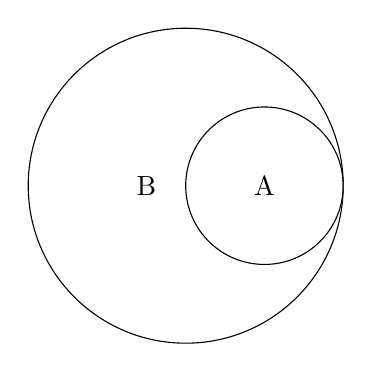
\begin{tikzpicture}
	\draw (0,0) circle (1cm);
	\draw (-1,0) circle (2cm);
	\node at (0,0) {A};
	\node at (-1.5, 0) {B};
\end{tikzpicture}

\ex{}{
	The set of integers with squares less than 100 is not a subset of the set of nonnegative integers
	because -1 is in the former set [as $\left( -1 \right) ^2 < 10$], but not the later set. The set of people who
	have taken discrete mathematics at your school is not a subset of the set of all computer science
	majors at your school if there is at least one student who has taken discrete mathematics who is
	not a computer science major.
}

\thm{}{
	For every set $S$
	\begin{enumerate}
		\item $\O \subseteq S$
		\item $S \subseteq S$
	\end{enumerate}

	\begin{enumerate}
		\item
		      \begin{myproof}
			      We will prove that $\O \subseteq S$, using a vacuous proof \\
			      Let $S$ be a set. \\
			      To show $\O \subseteq S$ we must show that $\forall x \left( x \in \O \to x \in S \right) $ is $T$. \\
			      Because $\O$ contains no elements $x \in  \O$ is always $F$ \\
			      This follows that the implication $x \in \O \to x \in S$ is always $T$ \\
			      Hence $\O \subseteq S$ \\
		      \end{myproof}
		\item
		      \begin{myproof}
			      We will prove that $S \subseteq S$, using a direct proof \\
			      Let $S$ be a set\\
			      To show $S \subseteq S$ we must show that $\forall x \left( x \in S \to x \in S \right) $ is $T$ \\
			      Assume $x \in S$ \\
			      Because $x \in S$ is always $T$, the implication $x \in S \to x \in S$ is always $T$ \\
			      $\therefore$ $\forall x \left( x \in S \to x \in S \right) $ is $T$\\
			      Hence $S \subseteq S$ \\
		      \end{myproof}

	\end{enumerate}
}

\dfn{Proper subset}{
	A set $A$ is \textit{proper subset} of a set $B$ if and only if every element of $A$ is also an element of $B$ and
	$A \neq B$. Denoted by $A \subset B$. I.e.
	\[
		\exists x \left( x \notin A \wedge x \in B \right) \wedge \forall x \left( x \in A \to x \in B \right)
	\]
	Is $T$.
}

\dfn{Further Equality}{
	Two sets $A$ and $B$ are equal if $A \subseteq B \wedge  B \subseteq A$ is $T$. I.e.
	$A = \left\{ \O, \left\{ a \right\}, \left\{ a \right\}, \left\{ b \right\}, \left\{ a, b \right\}     \right\}  $
	and $B = \left\{ x  \mid x \text{ is a subset of the set } \left\{ a,b \right\}  \right\}  $ are equal.
}

\subsection{Cardinality}

\dfn{Cardinality}{
	The number of distinct elements $n$ in a set $A$. Denoted by $\left| A \right| = n$.
	Where $n$ is a non-negative integer, we say that $A$ is a finite set.
}

\dfn{Infinite set}{
	A set $A$ is infinite if it is not finite. I.e. $\left| A \right| = \infty$
}


\subsection{Power Set}

\dfn{Power Set}{
	A set containing all the subsets of a given set $A$. Denoted by $\mathcal{P} \left( A \right) $. If a set has $n$
	distinct elements, then the cardinality of the power set is $2^{n}$.
}

\ex{}{
	\qs{}{
		What is the power set of the set $ \left\{ 0,1,2 \right\}  $
	}

	\sol{
		\[
			\mathcal{P}(\left\{ 0,1,2 \right\} ) = \left\{ \O, \left\{ 0 \right\}, \left\{ 1 \right\}, \left\{ 2 \right\},,
			\left\{ 0,1 \right\}, \left\{ 0, 2  \right\}, \left\{ 1,2 \right\}, \left\{ 0,1,2 \right\}        \right\}
		\]
	}
}

\ex{}{
	\qs{}{
		What is the power set of $\O$
	}

	\sol{
		\[
			\mathcal{P}(\O) = \left\{ \O \right\}
		\]
	}

	\qs{}{
		What is the power set of $\left\{ \O \right\} $
	}

	\sol{
		\[
			\mathcal{P}\left( \left\{ \O \right\}  \right) = \left\{ \O, \left\{ \O \right\}  \right\}
		\]
	}
}

\subsection{N-Tuples}
\dfn{Ordered N-Tuple}{
	N-tuple $\left( a_1, a_2, \ldots, a_n \right) $ is the ordered collection that has $a_1$ as its first element,
	$a_2$ as its second element, \ldots, and $a_n$ as its $n$th element.
}

Two n-tuples are equal if an only if each corresponding pair of their elements is equal, i.e. $\left( a_1, a_2, \ldots,
	a_n\right) = \left( b_1, b_2, \ldots, b_n \right)  $ are equal if and only if $a_i = b_i$, for $i = 1, 2,\ldots,n$.
\\

Ordered 2-tuples are called \textit{ordered pairs}. The ordered pairs, $\left( a, b \right) $ and $\left( c, d \right) $
are equal if and only if $a = c$ and $b = d$.


\subsection{Cartesian Products}

\dfn{Cartesian Product}{
	Let $A$ and $B$ be sets. The \textit{Cartesian Product} of $A$ and $B$, denoted by $A \times B$, is the set of all
	ordered pairs $\left( a, b \right) $, where $a \in A$ and $b \in B$. I.e.
	\[
		A \times B = \left\{ \left( a, b \right)  \mid a \in A \wedge b \in  B  \right\}
	\]
	The number of items in the Cartesian product of two sets is the product of the cardinality of each set.
}

\ex{}{
	\qs{}{
		What is the Cartesian product of $A = \left\{ 1, 2 \right\} $ and $B = \left\{ a, b, c \right\} $
	}

	\sol{
		\[
			A \times B = \left\{ \left( 1,a \right), \left( 1,b \right), \left( 1,c \right), \left( 2,a  \right),
			\left( 2,b \right), \left( 2, c \right)       \right\}
		\]
	}

	\qs{}{
		Show that the Cartesian product $B \times  A$ is not equal to the Cartesian product $A \times  B$.
	}

	\sol{
		\[
			B \times A = \left\{ \left( a, 1 \right) \left( a, 2 \right), \left( b, 1 \right), \left( b,2 \right), \left(
			c,1 \right), \left( c, 2 \right)       \right\}
		\]
		$\therefore A \times B \neq B \times A$
	}

}

\dfn{Cartesian Product of more than two sets}{
	The Cartesian product of the sets $A_1,A_2,\ldots,A_n$,denoted by $A_1 \times A_2 \times \ldots \times  A_n $,
	is the set of ordered $n$-tuples $\left( a_1,a_2, \ldots,a_n \right) $, where $a_i$ belongs to $A_i$ for $i =
		1,2,\ldots, n$. I.e.
	\[
		A_1\times A_2 \times \ldots \times A_n = \left\{ \left( a_1,a_2,\ldots a_n \right)  \mid a_i \in A_i \text{ for
		}  i = 1,2,\ldots,n  \right\}
	\]
}


\ex{}{
	\qs{}{
		What is the Cartesian product $A \times  B \times C$, where $A = \left\{ 0, 1 \right\} $, $B = \left\{ 1,2 \right\}
		$, $C = \left\{ 0,1,2 \right\} $.
	}

	\sol{
		\[
			A \times B \times C = \left\{ \left( 0,1,0 \right), \left( 0,1,1 \right), \left( 0,1,2 \right), \left( 0,2,0
			\right),  \left( 0,2,1 \right), \left( 0,2,2 \right), \left( 1,1,0 \right), \left( 1,1,1 \right) ,
			\left( 1,1,2\right),   \left( 1,2,0 \right), \left( 1,2,1 \right), \left( 1,2,2 \right)
			\right\}
		\]
	}
}

We use the notation $A^2$ to denote $A \times A$, the Cartesian product of $A$ and itself. Therefore
\[
	A^n = \left\{ \left( a_1, a_2,\ldots,a_n \right)  \mid a_i \in A \text{ for } i = 1,2,\ldots,n  \right\}
\]

\ex{}{
	Suppose $A = \left\{ 1,2 \right\} $. \\
	It follows $A^2 = \left\{ \left( 1,1 \right), \left( 1,2 \right), \left( 2,1
		\right), \left( 2,2 \right)     \right\} $, \\
	and $A^3 = \left\{ \left( 1,1,1 \right), \left( 1,1,2 \right),
		\left( 1,2,1 \right), \left( 1,2,2 \right), \left( 2,1,1 \right), \left( 2,1,2 \right), \left( 2,2,1 \right), \left(
		2,2,2\right)         \right\} $
}

\ex{}{
	\qs{}{
		What are the ordered pairs in the less than or equal to relation, which contains, $\left( a, b \right) $ if $a \leq
			b$, on the set $\left\{ 0,1,2,3 \right\} $
	}

	\sol{
		Let $R$ be the relation on the set $\left\{ 0,1,2,3  \right\} $, if $a \leq b$. \\
		\begin{align*}
			R = \left\{ \left( 0,0 \right), \left( 1,1 \right), \left( 2,2 \right), \left( 3,3 \right), \left( 0,1
			\right),  \left( 0,2 \right), \left( 0,3 \right), \left( 1,2 \right), \left( 1,3 \right), \left( 2,3 \right)            \right\}
		\end{align*}
	}
}

\subsection{Set Notation with Quantifiers}


We can restrict the domain of a quantifier to a set, I.e. Where $S$ is a set $\forall x \in S \left( P \left( x \right)
	\right) $, denotes the universal quantification of $P \left( x \right) $ for all elements in the set $S$. Which is
shorthand for $\forall x \left( x \in S \to P \left( x \right)  \right) $


\ex{}{
	$\forall x \in \mathbb{R} \left( x^2 \geq 0 \right) $ means "the square of any real number is greater than or equal
	to $0$". \\
	$\exists x \in \mathbb{Z} \left( x^2 = 1 \right) $ means "there exists an integer whose square is $1$"
}

\subsection{Truth Sets and Quantifiers}

\dfn{Truth Set}{
	For a predicate $P$ the truth set of $P$ is the set of all elements in the domain of discourse that make $P$ true.
	I.e. let $S$ be a set. The truth set of $P \left( x \right) $ is
	\[
		\left\{ x \in S  \mid  P \left( x \right)  \right\}
	\]
}

\ex{}{
	\qs{}{
		What are the truth set of the predicates $P \left( x \right) $, $Q \left( x \right) $, and $R \left( x \right)
		$, where the domain is the set of integers, and $P \left( x \right)\text{: }  | x | = 1 $, $Q \left( x
			\right)\text{: }
			x^2 = 2$, and $R \left( x \right)\text{: }  | x | = x  $
	}

	\sol{

		\noindent The truth set of $P$ is $\left\{ x \in \mathbb{Z}  \mid  |x| = 1 \right\} $ \\
		The truth set of $Q$ is $\left\{ x \in Z  \mid x^2 = 2 \right\} $ \\
		The truth set of $R$ is $\left\{ x \in \mathbb{Z}  \mid  |x| = x \right\} $
	}
}

\nt {
	$\forall x P \left( x \right) $ is $T$ over the domain $U$ if and only if the truth set of $P$ is $U$.
	\\
	$\exists x P \left( x \right) $ is $T$ over the domain $U$ if and only if the truth set of $P$ is not empty.
}

\section{Exercises}

\qs{}{
	List the members of these sets
	\begin{enumerate}
		\item $\left\{ x  \mid x \text{ is the square of an integer and } x < 100 \right\} $
		\item $\left\{ x  \mid x \text{ is an integer such that } x^2 = 2 \right\} $
	\end{enumerate}
}

\sol{
	\begin{enumerate}
		\item $\left\{ 1, 4, 9, 16, 25, 36, 49, 64, 81 \right\} $
		\item $\O$
	\end{enumerate}
}

\qs{}{
	Use set builder notation to describe the following sets
	\begin{enumerate}
		\item $\left\{ -3,-2,-1,0,1,2,3 \right\} $
		\item $\left\{ m,n,o,p \right\} $
	\end{enumerate}
}

\sol{
	\begin{enumerate}
		\item $\left\{ x  \mid -3 \leq x \leq 3  \right\} $
		\item $\left\{ x  \mid x \text{ is a letter in the word monopoly excluding "l" and "y" } \right\} $
	\end{enumerate}
}

\qs{}{
	Suppose that $A = \left\{ 2, 4, 6 \right\} $, $B = \left\{ 2, 6 \right\} $, $C = \left\{ 4, 6 \right\} $ and $D =
		\left\{ 4,6,8 \right\} $. Determine which of these sets are subsets of which other sets.
}

\sol{
	\begin{align*}
		B \subseteq  A \\
		C \subseteq A  \\
		C \subseteq D  \\
	\end{align*}
}

\qs{}{
	Suppose that $A$, $B$, $C$, are sets such that $A \subseteq B$ and $B \subseteq C$. Show that $A \subseteq C$
}

\sol{

	\begin{align*}
		A \subseteq B  \text{ means } \forall x \left( x \in A \to x \in  B \right) \\
		B \subseteq C \text{ means } \forall x \left( x \in B \to x \in C \right)   \\
		A \subseteq C \text{ means } \forall x \left( x \in A \to x \in  C \right)  \\
	\end{align*}

	\begin{align*}
		\begin{deduction}
			\premise{ \forall x \left( x \in  A \to x \in  B \right)  }
			\premise{ \forall x \left( x \in  B \to x \in C \right) }
			\conclusion{ \forall x \left( x \in A \to x \in C \right) }
		\end{deduction}
	\end{align*}

	\gdef\rownumber{\stepcounter{magicrownumbers}\arabic{magicrownumbers}}
	\begin{table}[h!]
		\begin{center}
			\begin{tabular}{ | @{\makebox[3em][r]{\rownumber\space}} | c | c | }
				\hline
				\multicolumn{1}{ | @{\makebox[3em][r]{~}} |c| }{Steps} & \multicolumn{1}{|c|}{Reasons}        \\
				\hline
				\hline
				$ \forall x \left( x \in  A \to x \in  B \right)  $    & Premise 1                            \\
				$ \forall x \left( x \in  B \to x \in C \right) $      & Premise 2                            \\
				$x \in  A \to x \in  B$                                & Universal Instantiation of 1         \\
				$x \in B \to x \in C$                                  & Universal Instantiation of 2         \\
				$x \in A \to x \in C$                                  & By Hypothetical Syllogism of 3 and 4 \\
				$\forall x \left( x \in A \to x \in C \right) $        & Universal generalization of 5        \\
				\hline
			\end{tabular}
		\end{center}
	\end{table}
}

\qs{}{
	Find the power set of each of these sets, where $a$ and $b$ are distinct elements.
	\begin{enumerate}
		\item $\{a\} $
		\item $\{a, b\} $
		\item $\{\O, \{\O\} \} $
	\end{enumerate}
}

\sol{
	\begin{enumerate}
		\item $\mathcal{P}\left( \{a\}  \right)  = \{\O, \{a\} \} $
		\item $\mathcal{P}(\{a,b\} ) = \{\O, \{a\}, \{b\}, \{a,b\}   \} $
		\item $\mathcal{P}(\{\O, \{\O\} \} ) = \{\O, \{\O\}\, \{\{\O\} \}, \{\O, \{\O\} \}   \} $
	\end{enumerate}
}


\chapter{Set Operations}

\section{Set Operations}

\subsection{Union}

\dfn{Union}{
	Let $A$ and $B$ be sets. The \textit{union} of $A$ and $B$, denoted by $A \cup B$, is the set of all elements that
	are either in $A$ or in $B$ or in both. I.e.
	\[
		A \cup B = \left\{ x  \mid  x \in A \vee x \in B \right\}
	\]
}

\subsection{Intersection}

\dfn{Intersection}{
	Let $A$ and $B$ be sets. The \textit{intersection} of $A$ and $B$, denoted by $A \cap B$, is the set of all elements
	that are in both $A$ and $B$. I.e.
	\[
		A \cap B = \left\{ x  \mid  x \in A \wedge x \in B \right\}
	\]
}

\subsection{Complement}

\dfn{Complement}{
	Let $A$ be a set. The \textit{complement} of the set A (with respect to $U$), denoted by $\overline{A}$ is the set
	$U - A$. I.e.
	\[
		\overline{A} = \left\{ x \in U  \mid x \notin A \right\}
	\]
}

\subsection{Difference}

\dfn{Difference}{
	Let $A$ and $B$ be sets.  The \textit{difference} of $A$ and $B$, denoted by $A - B$, is the set of all elements
	that are in $A$ but not in $B$. I.e.
	\[
		A - B = \left\{ x  \mid  x \in A \wedge x \notin B \right\}
	\]
	Or
	\[
		A - B = A \cap \overline{B}
	\]
}

\subsection{Symmetric Difference}

\dfn{Symmetric Difference}{
	Let $A$ and $B$ be sets. The \textit{symmetric difference} of $A$ and $B$, denoted by $A \oplus  B$, is the set
	of all elements that are in exactly one of $A$ and $B$. I.e.
	\[
		A \oplus B = \left( A - B \right) \cup \left( B - A\right)
	\]
}

\ex{}{
	\qs{}{
		\begin{align*}
			U = \left\{ 0,1,2,3,4,5,6,7,8,9,10 \right\} \\
			A = \left\{ 1,2,3,4,5 \right\}              \\
			B = \left( 4,5,6,7,8 \right)
		\end{align*}
		What is $A \oplus B$
	}

	\sol{
		\[
			A \oplus B = \left\{ 1,2,3,6,7,8 \right\}
		\]
	}
}

\subsection{The Cardinality of the Union of Two Sets}

The cardinality of the union of two sets $A$ and $B$ is given by
\[
	\left| A \cup B \right| = \left| A \right| + \left| B \right| - \left| A \cap B \right|
\]

\section{Set Identities}

\subsection{Identity Laws}

\begin{align*}
	A \cap   U = A \\
	A \cup  \O = A
\end{align*}

\subsection{Domination Laws}

\begin{align*}
	A \cup U = U \\
	A \cap \O = \O
\end{align*}

\subsection{Idempotent Laws}

\begin{align*}
	A \cup A = A \\
	A \cap A = A
\end{align*}

\subsection{Complementation Law}
\[
	\overline{\left( \overline{A} \right) } = A
\]

\subsection{Commutative Laws}

\begin{align*}
	A \cup B = B \cup A \\
	A \cap B = B \cap A
\end{align*}

\subsection{Associative Laws}

\begin{align*}
	A \cup \left( B \cup  C \right)  = \left( A \cup B \right)  \cup C \\
	A \cap \left( B \cap C  \right)  = \left( A \cap B \right)  \cap C
\end{align*}

\subsection{Distributive Laws}

\begin{align*}
	A \cup \left( B \cap C \right)  = \left( A \cup B \right)  \cap \left( A \cup C \right) \\
	A \cap \left( B \cup C  \right)  = \left( A \cap B \right)  \cup \left( A \cap C \right)
\end{align*}

\subsection{De Morgan's Laws}
\begin{align*}
	\overline{A \cap  B} = \overline{A} \cup \overline{B} \\
	\overline{A \cup B } = \overline{A} \cap \overline{B}
\end{align*}

\subsection{Absorption Laws}
\begin{align*}
	A \cup \left( A \cap B \right) = A \\
	A \cap  \left( A \cup B  \right)  = A
\end{align*}

\subsection{Complement Laws}
\begin{align*}
	A \cup \overline{A} = U \\
	A \cap \overline{A} = \O
\end{align*}

\subsection{Proving Set Identities}

There are different ways to prove set identities, these include:
\begin{itemize}
	\item Proving each set is a subset of the other
	\item Using set builder notation and propositional logic
	\item Using Membership tables
\end{itemize}

\dfn{Membership Table}{
	A table that shows the truth value of a predicate for all possible combinations of truth values of its variables.
}


\ex{}{
	\qs{}{
		Prove that
		\[
			\overline{A \cap B} = \overline{A} \cup \overline{B}
		\]
	}

	\noindent Using propositional logic:
	\begin{myproof}
		We prove this identity by showing that each set is a subset of the other. I.e.\\
		\[
			\overline{A \cap  B} \subseteq \overline{A} \cup  \overline{B} \wedge \overline{A} \cap \overline{B} \subseteq
			\overline{A \cap B}
		\]
		\begin{align*}
			\overline{A \cap B} \subseteq \overline{A} \cup \overline{B} \text{ means } \forall x \left( x \in
			\overline{A \cap B} \to x \in \overline{A} \cup  \overline{B} \right) \\
			\overline{A} \cup \overline{B} \subseteq \overline{A \cap B} \text{ means } \forall x \left( x \in
			\overline{A} \cup \overline{B} \to x \in \overline{A \cap B} \right)  \\
		\end{align*}
		Assume that $x \in  \overline{A \cap  B}$\\
		\begin{align*}
			x \in  \overline{A \cap B}                               \tag*{Assumption}            \\
			x \notin A \cap B                                     \tag*{Definition of Complement} \\
			\neg \left( x \in A \cap B \right)                    \tag*{Definition of $\notin$ }  \\
			\neg \left( x \in A \wedge x \in B \right)   \tag*{Definition of intersection}        \\
			\neg \left( x \in A \right) \vee \neg \left( x \in  B  \right) \tag*{ By First De Moragn's Law for propositional
			logic}                                                                                \\
			x \notin A \vee x \notin B \tag*{Definition of Complement}                            \\
			x \in \overline{A} \cup \overline{B} \tag*{Definition of union}
		\end{align*}
		Then we assume $x \in \overline{A} \cup \overline{B}$
		\begin{align*}
			x \in \overline{A} \cup \overline{B} \tag*{Assumption}                                               \\
			x \notin A \vee x \notin B \tag*{Definition of union}                                                \\
			\neg \left( x \in A \right)  \vee  \neg \left( x \in B \right)  \tag*{Definition of Complement}      \\
			\neg \left( x \in A \wedge  x \in B \right) \tag*{By Second De Morgan's Law for propositional logic} \\
			x \notin A \wedge x \notin B \tag*{Definition of Complement}                                         \\
			x \notin A \cap B \tag*{Definition of intersection}                                                  \\
			x \in \overline{A \cap B} \tag*{Definition of Complement}
		\end{align*}

	\end{myproof}
	\noindent Using set builder notation
	\begin{align*}
		\overline{A \cap B} & = \{ x  \mid x \notin A \cap B\} \tag*{Definition of Complement}                                                \\
		                    & = \{x  \mid \neg \left( x \in \left( A \cap B \right)  \right) \} \tag*{Definition of $\notin$}                 \\
		                    & = \{x  \mid \neg \left( x \in A \wedge x \in B \right) \} \tag*{Definition of Intersection}                     \\
		                    & = \{x  \mid \neg \left( x \in A \right) \vee \neg \left( x \in B \right)  \} \tag*{By First De Morgan's Law for
		propositional logic}                                                                                                                  \\
		                    & = \{x  \mid x \notin A \vee x \notin B\} \tag*{Definition of Complement}                                        \\
		                    & = \{x | x \in \overline{A} \cup \overline{B}\} \tag*{Definition of union}                                       \\
		                    & = \overline{A} \cup \overline{B}                                                                                \\
	\end{align*}
}

\section{Generalized Unions and Intersections}

\dfn{Generalized Union}{
	The union of a collection of sets  that contains those elements that are members of at least one set in the
	collection. Denoted by
	\[
		A_1 \cup A_2 \cup \ldots \cup A_n = \bigcup_{i = 1} ^n A_i
	\]
	Where $A_1 \cup A_2 \cup  \ldots A_n$ is the union of sets $A_1,A_2,\ldots,A_n$
}

\dfn{Generalized Intersection}{
	The intersection of a collection of sets that contains those elements that are members of all the sets in the
	collection. Denoted by
	\[
		A_1 \cap A_2 \cap \ldots A_n = \bigcap_{i = 1} ^n A_i
	\]
	Where $A_1 \cap A_2 \cap \ldots \cap A_n$ is the intersection of sets $A_1,A_2,\ldots,A_n$
}

\ex{}{
	For $i = 1,2,\ldots,$ let $A_i = \{i,i+1,i+2,\ldots\} $. Then.
	\[
		\bigcup_{i = 1} ^n A_i = \bigcup_{i = 1} ^n \{i, i+1, i+2,\ldots\} = \{1,2,3,\ldots\}
	\]
	and
	\[
		\bigcap_{i = 1} ^{n}A_i = \bigcap_{i = 1} ^{n}\{i,i+1,i+2,\ldots\} = \{n, n+1, n+2\} = A_n
	\]
}

We can extend this notation to other families of sets I.e.
\[
	A_1 \cup A_2 \cup \ldots \cup A_n \cup \ldots = \bigcup_{i = 1} ^{\infty}A_i
\]
Denotes the union of the sets $A_1,A_2,\ldots,A_n,\ldots$, and the intersection of these sets is denoted by
\[
	A_1 \cap A_2 \cap \ldots \cap A_n \cap \ldots = \bigcap_{i = 1} ^{\infty}A_i
\]

Generally when $I$ is set, the notations $\bigcap_{i \in  I}A_i $ and $\bigcup_{i \in  I}A_i $ are used to denote the
intersection and union of the sets $A_i$ for $i \in I$, respectively, where
\[
	\bigcap_{i \in  I} A_i = \{x  \mid \forall i \in I \left( x \in A_i \right) \}
\]
and
\[
	\bigcup_{i \in  I}  A_i = \{x  \mid \exists i \in I \left( x \in A_i \right) \}
\]

\ex{}{
	Suppose $A_i = \{1,2,3,\ldots,i\} $ for $i = \{1,2,3,\ldots\} $ Then
	\[
		\bigcup_{i = 1} ^{\infty} A_i = \bigcup_{i = 1}^{\infty}  \{1,2,3,\ldots,i\}  = \mathbb{Z}^{+}
	\]

	and
	\[
		\bigcap_{i = 1} ^{\infty}A_i = \bigcap_{i = 1} ^{\infty} \{1,2,3,\ldots,i\}  = \{1\}
	\]
}

\section{Exercises}

\qs{}{
	List the members of these sets
	\begin{enumerate}
		\item  $\left\{ x  \mid x \text{ is a real number such that } x^2 = 1 \right\}$
		\item $\{x | x \text{ is a positive integer less than 12}\} $
		\item $\{x | x \text{ is the square of an integer and } x < 100\} $
		\item $ \left\{ x  \mid  x \text{ is an integer such that } x^2 = 2 \right\} $
	\end{enumerate}
}

\sol{
	\begin{enumerate}
		\item $\left\{ -1, 1 \right\} $
		\item
		\item
		\item $ \O $
	\end{enumerate}
}

\qs{}{
	Use set builder notation to show that:
	\begin{enumerate}
		\item $A \cup U = U$
		\item $A \cap \O = \O$
		\item $A \cup  \overline{A} = U$
		\item $A \cap \overline{A} = \O$
	\end{enumerate}
}

\sol{
	\begin{enumerate}
		\item
		      \begin{align*}
			      A \cup U & = \{ x  \mid x \in A \cup U\} \tag*{Set builder notation}         \\
			               & = \{x  \mid x \in A \vee   x \in U \} \tag*{Definition of Union}  \\
			               & = \{x  \mid  x \in A \vee  T\} \tag*{Definition of Universal Set} \\
			               & = \{x  \mid T \} \tag*{By Domination law for propositional logic} \\
			               & = U \tag*{Definition of Universal Set}                            \\
		      \end{align*}
		\item
		\item
		\item
		      \begin{align*}
			      A \cap \overline{A} & = \{ x  \mid x \in A \cap \overline{A}\} \tag*{Set builder notation}                     \\
			                          & = \{x  \mid x \in A \wedge x \in \overline{A} \} \tag*{Definition of intersection}       \\
			                          & = \{x  \mid x \in A \wedge \left( x \notin A \right)  \} \tag*{Definition of Complement} \\
			                          & = \{x | x \in A \wedge  \neg \left( x \in  A \right) \} \tag*{Definition of $\O$}        \\
			                          & = \{x  \mid F\} \tag*{By Identity law of propositional logic}                            \\
			                          & = \O \tag*{Definition of $\O$}                                                           \\
		      \end{align*}
	\end{enumerate}
}

\qs{}{
	Let $A$ and $B$ be sets. Show that
	\begin{enumerate}
		\item $\left( A \cap B \right) \subseteq A $
		\item $A \subseteq \left( A \cup B \right) $
		\item $A \subseteq \left( A \cup B \right) $
		\item $A - B \subseteq A$
		\item $A \cap \left( B - A \right) = \O $
		\item $A \cup \left( B - A \right) = A \cup B $
	\end{enumerate}
}

\sol{
	\begin{enumerate}
		\item
		      \begin{align*}
			      \left( A \cap B \right) \subseteq A \text{ means } \forall x \left( x \in \left( A \cap B \right) \to x \in A  \right)
		      \end{align*}
		      Assume $x \in \left( A \cap B \right) $
		      \gdef\rownumber{\stepcounter{magicrownumbers}\arabic{magicrownumbers}}
		      \begin{table}[h!]
			      \begin{center}
				      \begin{tabular}{ | @{\makebox[3em][r]{\rownumber\space}} | c | c | }
					      \hline
					      \multicolumn{1}{ | @{\makebox[3em][r]{~}} |c| }{Steps} & \multicolumn{1}{|c|}{Reasons} \\
					      \hline
					      \hline
					      $x \in A \cap B$                                       & Assumption                    \\
					      $x \in A \wedge x \in B$                               & Definition of intersection    \\
					      $x \in A$                                              & Simplification of 2           \\
					      \hline
				      \end{tabular}
			      \end{center}
		      \end{table}
		      \\
		      $\therefore$ $x \in \left( A \cap B \right) \to x \in A $\\
		      Conclusion: $\left( A \cap B \right) \subseteq A $
		\item
		      \begin{myproof}
			      \[
				      A \subseteq \left( A \cup B \right)  \text{ means } \forall x \left( x \in A \to x \in A \cup B \right)
			      \]
			      \gdef\rownumber{\stepcounter{magicrownumbers}\arabic{magicrownumbers}}
			      \begin{table}[h!]
				      \begin{center}
					      \begin{tabular}{ | @{\makebox[3em][r]{\rownumber\space}} | c | c | }
						      \hline
						      \multicolumn{1}{ | @{\makebox[3em][r]{~}} |c| }{Steps} & \multicolumn{1}{|c|}{Reasons} \\
						      \hline
						      \hline
						      $x \in A$                                              & Premise                       \\
						      $x \in A \wedge x \in B$                               & Addition                      \\
						      $x \in A \cup B $                                      & Definition of Union           \\
						      \hline
					      \end{tabular}
				      \end{center}
			      \end{table}\\
			      $\therefore$ $x \in A \to x \in A \cup B$\\
			      Conclusion: $A \subseteq A \cup B$
		      \end{myproof}
		\item
		      \begin{myproof}

		      \end{myproof}

		\item
		      \begin{myproof}

		      \end{myproof}

		\item
		      \begin{myproof}

		      \end{myproof}

		\item
		      \begin{myproof}

		      \end{myproof}

	\end{enumerate}
}

\qs{}{
	Show that if $A$ is a subset of a universal set $U$, then
	\begin{enumerate}
		\item $A \oplus A = \O$
		\item $A \oplus  \O = A$
		\item $A \oplus U = \overline{A}$
		\item $A \oplus \overline{A} = U$
	\end{enumerate}
}

\sol{
	\begin{enumerate}
		\item
		      \begin{align*}
			      A \oplus A & = \left( A - A \right)  \cup \left( A - A \right) \tag*{Definition of Symmetric Difference}        \\
			                 & = \{x  \mid  \left( x \in A \wedge x \notin A \right) \cup \left( x \in A \wedge x \notin A
			      \right)  \} \tag*{Definition of Difference}                                                                     \\
			                 & = \{x  \mid  \left( x \in A \wedge x \in \overline{A} \right) \cup  \left( x \in A \wedge
			      x \in \overline{A}\right)  \} \tag*{Definition of Complement}
			      \\
			                 & = \{x  \mid \left( x \in A \cap \overline{A} \right)\cup  \left( x \in A \cap \overline{A} \right)
			      \} \tag*{Definition of Intersection}                                                                            \\
			                 & = \{x  \mid \O \cup \O\} \tag*{By Second Complement Law}                                           \\
			                 & = \{x  \mid \O \} \tag*{By First Idempotent Law}                                                   \\
			                 & = \O \tag*{By Definition of $\O$}                                                                  \\
		      \end{align*}
	\end{enumerate}
}

\end{document}
